\subsection{The action of $\PSL{\Z}$ on $\EC$}

In Theorem~\ref{thm_SL2FunDomAlg} we have seen an algorithm which naturally gives rise to a set $\hat{\mathcal{R}} \subseteq \C^2$ which can easily be restricted to a subset $\hat{\mathcal{F}} \subseteq \hat{\mathcal{R}}$ being a fundamental region for the action of $\SL{\Z}$ on $\hat{\mathcal{S}}$. We can exploit this fact in search of a fundamental region for the action on of the (inhomogeneous) modular group $\PSL{\Z}$ on $\EC$. For this purpose we project $\C^2$ onto $\EC$ using the map $\pi : \C^2 \to \EC$,
\begin{equation}
\pi : \cvec{u}{v} \mapsto \frac{u}{v}.
\end{equation}
Let us first consider image of $\hat{\mathcal{S}}$ under $\pi$. If $({}^u_v) \in \hat{\mathcal{S}}$, then by definition $u$ and $v$ are linear independent over $\R$ or linear dependent over $\Q$. In the first case we have $\frac{u}{v} \in \C \setminus \R$ and in the second case $\frac{u}{v} \in \Q \cup \{\infty\}$. This means $\frac{u}{v}$ may be everything but irrational. Denoting set of irrational numbers by $\Irrat = \R \setminus \Q$, we thus have
\begin{equation*}
\pi(\hat{\mathcal{S}}) = \EC \setminus \Irrat.
\end{equation*}
Projection of the set $\hat{\mathcal{R}} \subseteq \C^2$ leads to the region $\mathcal{R} \subseteq \EC$ (see also Figure~\ref{fig_PSL2MinRegion}),
\begin{equation}
\mathcal{R} := \pi\left(\hat{\mathcal{R}}\right) = 
\setdefsz{\Big}{\frac{u}{v} \in \EC}{\abs{u\conj{v} + \conj{u}v} < \min\{\abs{u}^2, \abs{v}^2\}}.
\end{equation}
\begin{figure}
\centering
\includegraphics[width=0.8\textwidth]{figures/minimal-region}
\caption{The region $\mathcal{R}$ of numbers $z = u/v \in \EC$ with $\abs{u\conj{v} + \conj{u}v} < \min\{\abs{u}^2,\abs{v}^2\}$. It is obtained by taking the strip $\setdef{z \in \C}{\Re{z} \in \left(-\reci{2},\reci{2}\right)}$  and cutting out two closed disks of unit radius centered about the real points $\pm 1$. The arising vertices are labeled. As usual, $T$ is the transformation $z \mapsto -\reci{z}$ and $\rho = \exp(2 \pi \ii / 3)$ is a third root of unity.}
\label{fig_PSL2MinRegion}
\end{figure}
It follows that $\mathcal{R}$ contains a fundamental region $\mathcal{F}$ for the action of $\PSL{\Z}$ on $\EC \setminus \Irrat$. As in the homogeneous case, we see from Theorem~\ref{thm_SL2FunDomGlobMin} that equivalence of points within $\mathcal{R}$ can be established only by powers of the transformation $T \in \PSL{\Z}$. Since $T^2 = 1$, this means that in order to obtain a fundamental region we just need to choose for each $z \in \mathcal{R}$ only between one of the equivalent points $z$ and $Tz$. This can for example be done such that $\abs{z} > 1$.
\begin{corollary}
The set
\begin{equation}
\mathcal{F} := \setdefsz{\bigg}{z \in \C}{\abs{\Re{z}} < \reci{2} \text{ and } \abs{z} > 1}
\end{equation}
is a fundamental region for the action of the inhomogeneous modular group $\PSL{\Z}$ on $\EC \setminus \Irrat$.
\end{corollary}
\begin{proof}
First observe that $\mathcal{F}$ is exactly the set
\begin{equation*}
\mathcal{F} = \mathcal{R} \cap \setdef{z \in \C}{\abs{z} > 1},
\end{equation*}
compare also Figure~\ref{fig_PSL2MinRegion}. Obviously $\mathcal{F}$ is a nonempty subset of $\mathcal{R}$, which is why two distinct points of $\mathcal{F}$ can be equivalent only by the transformation $T$. However, since $\abs{z} > 1$ implies $\abs{Tz} = \abs{-1/z} < 1$, this cannot be the case. Hence $\mathcal{F}$ contains no equivalent distinct points.

It remains to show that every $z = \frac{u}{v} \in \mathcal{S}$ is equivalent to a point of the topological closure $\topcl{\mathcal{F}}$. For this purpose apply the algorithm of Theorem~\ref{thm_SL2FunDomAlg} to the vector $({}^u_v)$ in order to obtain a transformation $B \in \PSL{\Z}$ which maps $z$ to a point of $\topcl{\mathcal{R}}$. It then follows that at least one of the points $Bz$ or $TBz$ lies in $\topcl{\mathcal{F}}$.
\end{proof}

\begin{figure}
\centering
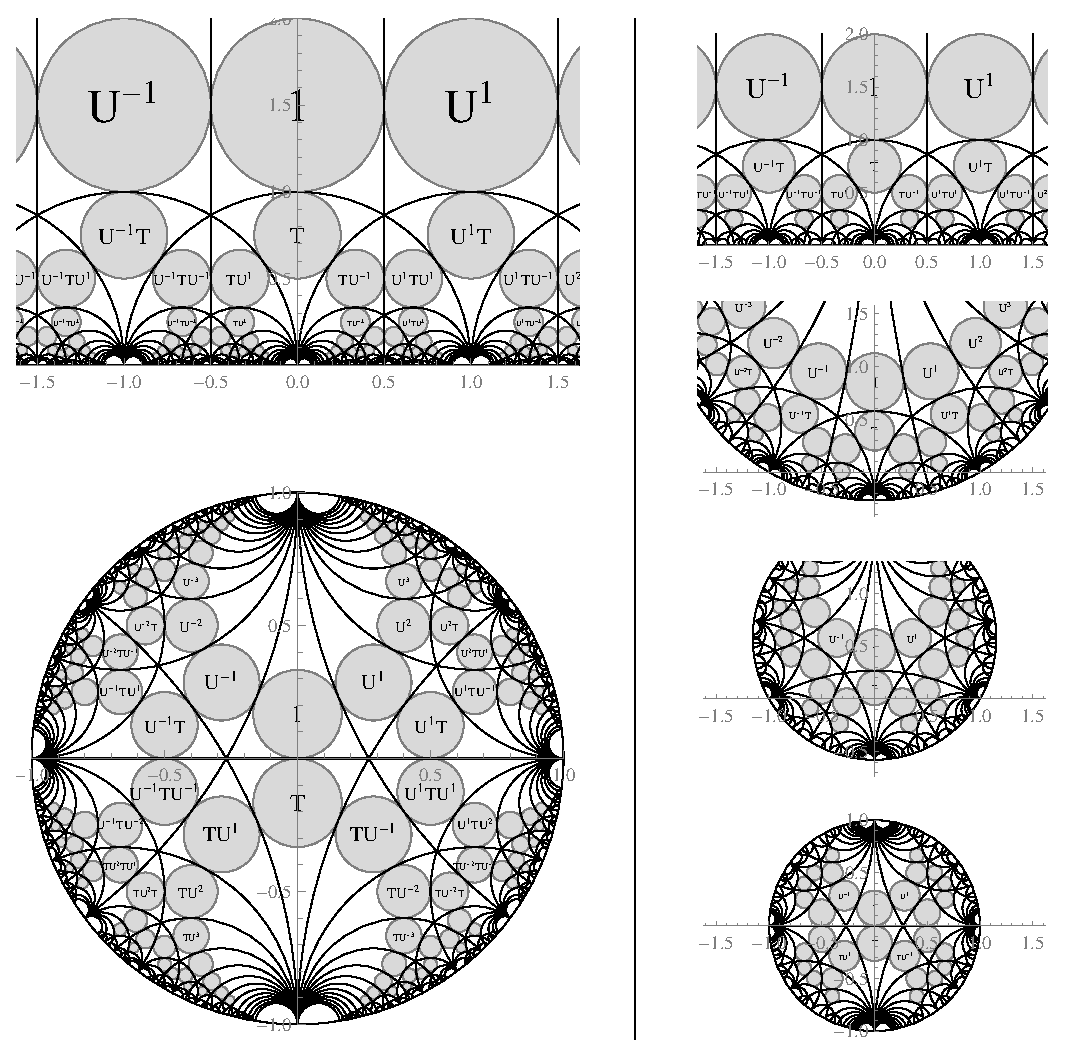
\includegraphics[width=\textwidth]{figures/modular-tiling-1}
\caption{The tessellation of the upper halfplane.}
\label{fig_ModularTiling}
\end{figure}
